\documentclass{standalone}
\usepackage{tikz}
\usetikzlibrary{patterns}
\usetikzlibrary{positioning}
\usetikzlibrary{patterns, positioning}
\usetikzlibrary{shapes.misc}
\usepackage[outline]{contour}
\contourlength{1.5pt} 
\usetikzlibrary{calc}
        \usepackage{relsize}
        \tikzset{fontscale/.style = {font=\relsize{#1}}}

\begin{document}
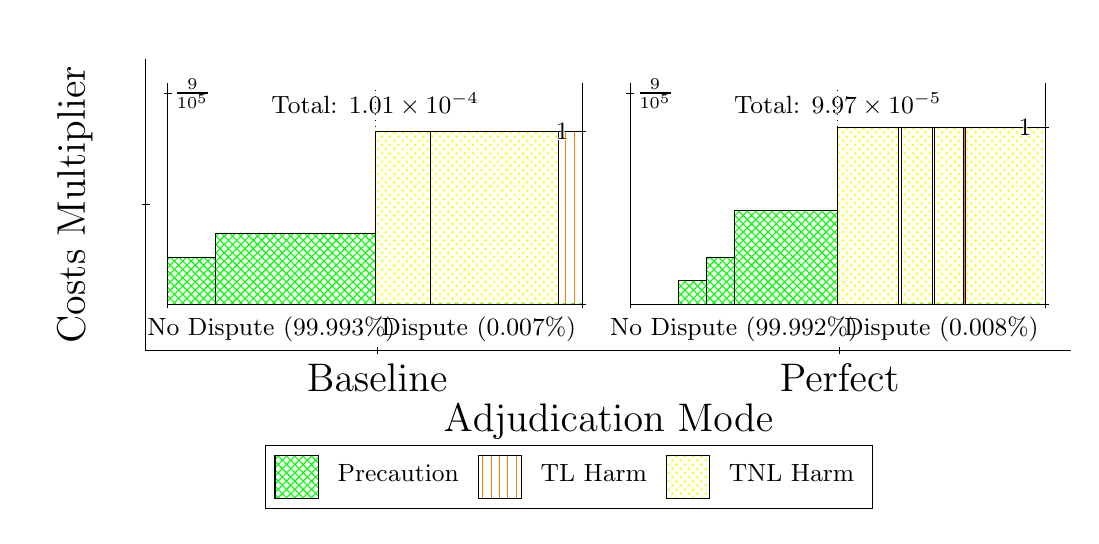
\begin{tikzpicture}
\clip(-0.5,-1.1) rectangle +(13.25,6.2);
\draw[black] (1,1) -- (1,4.7);
\node[rotate=90, fontscale=2, anchor=center] at (0.1, 2.85) {Costs Multiplier};
\draw[black] (0.95,2.85) -- (1.05,2.85);
\node[fontscale=2, anchor=east] at (0.95, 2.85) { };

\draw[black] (1,1) -- (12.75,1);
\node[fontscale=2, anchor=center] at (6.875, 0.1) {Adjudication Mode};
\draw[black] (3.9375,0.95) -- (3.9375,1.05);
\node[fontscale=2, anchor=north] at (3.9375, 0.95) {Baseline};
\draw[black] (9.8125,0.95) -- (9.8125,1.05);
\node[fontscale=2, anchor=north] at (9.8125, 0.95) {Perfect};


\draw[pattern=crosshatch, pattern color=green,draw=black,very thin] (1.279,1.592) rectangle (1.8847,2.1862);
\draw[pattern=crosshatch, pattern color=green,draw=black,very thin] (1.8847,1.592) rectangle (3.9125,2.4833);
\draw[pattern=crosshatch, pattern color=green,draw=black,very thin] (3.9125,1.592) rectangle (4.6174,1.592);
\draw[pattern=crosshatch dots, pattern color=yellow,draw=black,very thin] (3.9125,1.592) rectangle (4.6174,3.7824);
\draw[pattern=crosshatch, pattern color=green,draw=black,very thin] (4.6174,1.592) rectangle (4.6182,1.592);
\draw[pattern=vertical lines, pattern color=orange,draw=black,very thin] (4.6174,1.592) rectangle (4.6182,3.7824);
\draw[pattern=crosshatch, pattern color=green,draw=black,very thin] (4.6182,1.592) rectangle (6.2435,1.5921);
\draw[pattern=crosshatch dots, pattern color=yellow,draw=black,very thin] (4.6182,1.5921) rectangle (6.2435,3.7824);
\draw[pattern=crosshatch, pattern color=green,draw=black,very thin] (6.2435,1.592) rectangle (6.546,1.5921);
\draw[pattern=vertical lines, pattern color=orange,draw=black,very thin] (6.2435,1.5921) rectangle (6.546,3.7824);
\node[font=\small,text=black,anchor=north] at (3.9125, 4.4) {Total: $1.01\times 10^{-4}$};
\draw[black,very thin] (1.279,1.592) -- (1.279,4.4);
\draw[black,very thin] (1.229,4.2658) -- (1.329,4.2658);
\node[font=\small,text=black, anchor=west] at (1.229, 4.2658) {$\frac{9}{10^{5}}$};

\draw[black,dotted,very thin] (3.9125,1.6762) -- (3.9125,4.3158);
\draw[black,very thin] (6.546,1.592) -- (6.546,4.4);
\draw[black,very thin] (6.496,1.592) -- (6.596,1.592);
\node[font=\small,text=black, anchor=east] at (6.496, 1.592) {\contour{white}{}};
\draw[black,very thin] (6.496,3.7823) -- (6.596,3.7823);
\node[font=\small,text=black, anchor=east] at (6.496, 3.7823) {\contour{white}{1}};

\draw[black,very thin] (1.279,1.592) -- (6.546,1.592);
\draw[black,very thin] (1.279,1.542) -- (1.279,1.642);
\node[font=\small,text=black, anchor=north] at (1.279, 1.542) {};
\draw[black,very thin] (6.546,1.542) -- (6.546,1.642);
\node[font=\small,text=black, anchor=north] at (6.546, 1.542) {};

\node[font=\small,text=black,anchor=south] at (2.5958, 0.992) {No\ Dispute\ (99.993\%)};
\node[font=\small,text=black,anchor=south] at (5.2293, 0.992) {Dispute\ (0.007\%)};

\draw[pattern=crosshatch, pattern color=green,draw=black,very thin] (7.7597,1.592) rectangle (8.1155,1.8891);
\draw[pattern=crosshatch, pattern color=green,draw=black,very thin] (8.1155,1.592) rectangle (8.4707,2.1862);
\draw[pattern=crosshatch, pattern color=green,draw=black,very thin] (8.4707,1.592) rectangle (9.7875,2.7803);
\draw[pattern=crosshatch dots, pattern color=yellow,draw=black,very thin] (9.7875,1.592) rectangle (10.556,3.8383);
\draw[pattern=vertical lines, pattern color=orange,draw=black,very thin] (10.556,1.592) rectangle (10.589,3.8383);
\draw[pattern=crosshatch, pattern color=green,draw=black,very thin] (10.589,1.592) rectangle (10.994,1.592);
\draw[pattern=crosshatch dots, pattern color=yellow,draw=black,very thin] (10.589,1.592) rectangle (10.994,3.8383);
\draw[pattern=crosshatch, pattern color=green,draw=black,very thin] (10.994,1.592) rectangle (11.019,1.592);
\draw[pattern=vertical lines, pattern color=orange,draw=black,very thin] (10.994,1.592) rectangle (11.019,3.8383);
\draw[pattern=crosshatch, pattern color=green,draw=black,very thin] (11.019,1.592) rectangle (11.378,1.592);
\draw[pattern=crosshatch dots, pattern color=yellow,draw=black,very thin] (11.019,1.592) rectangle (11.378,3.8384);
\draw[pattern=crosshatch, pattern color=green,draw=black,very thin] (11.378,1.592) rectangle (11.402,1.592);
\draw[pattern=vertical lines, pattern color=orange,draw=black,very thin] (11.378,1.592) rectangle (11.402,3.8384);
\draw[pattern=crosshatch, pattern color=green,draw=black,very thin] (11.402,1.592) rectangle (12.421,1.5921);
\draw[pattern=crosshatch dots, pattern color=yellow,draw=black,very thin] (11.402,1.5921) rectangle (12.421,3.8384);
\node[font=\small,text=black,anchor=north] at (9.7875, 4.4) {Total: $9.97\times 10^{-5}$};
\draw[black,very thin] (7.154,1.592) -- (7.154,4.4);
\draw[black,very thin] (7.104,4.2658) -- (7.204,4.2658);
\node[font=\small,text=black, anchor=west] at (7.104, 4.2658) {$\frac{9}{10^{5}}$};

\draw[black,dotted,very thin] (9.7875,1.6762) -- (9.7875,4.3158);
\draw[black,very thin] (12.421,1.592) -- (12.421,4.4);
\draw[black,very thin] (12.371,1.592) -- (12.471,1.592);
\node[font=\small,text=black, anchor=east] at (12.371, 1.592) {\contour{white}{}};
\draw[black,very thin] (12.371,3.8383) -- (12.471,3.8383);
\node[font=\small,text=black, anchor=east] at (12.371, 3.8383) {\contour{white}{1}};

\draw[black,very thin] (7.154,1.592) -- (12.421,1.592);
\draw[black,very thin] (7.154,1.542) -- (7.154,1.642);
\node[font=\small,text=black, anchor=north] at (7.154, 1.542) {};
\draw[black,very thin] (12.421,1.542) -- (12.421,1.642);
\node[font=\small,text=black, anchor=north] at (12.421, 1.542) {};

\node[font=\small,text=black,anchor=south] at (8.4708, 0.992) {No\ Dispute\ (99.992\%)};
\node[font=\small,text=black,anchor=south] at (11.104, 0.992) {Dispute\ (0.008\%)};

\coordinate (LegendAnchor) at (6.375,0);
\begin{scope}[align=center]
\matrix[scale=0.6,draw=black,below=0.2cm of LegendAnchor,nodes={draw},column sep=0.12cm]{
\node[rectangle,draw,minimum width=0.55cm,minimum height=0.55cm,pattern=crosshatch, pattern color=green]{}; &
        \node[draw=none,font=\small]{Precaution}; &
\node[rectangle,draw,minimum width=0.55cm,minimum height=0.55cm,pattern=vertical lines, pattern color=orange]{}; &
        \node[draw=none,font=\small]{TL Harm}; &
\node[rectangle,draw,minimum width=0.55cm,minimum height=0.55cm,pattern=crosshatch dots, pattern color=yellow]{}; &
        \node[draw=none,font=\small]{TNL Harm}; \\
};\end{scope}

\end{tikzpicture}
\end{document}